\documentclass[11pt,a4paper]{article}
\usepackage[utf8]{inputenc}
\usepackage[T1]{fontenc}
\usepackage{lmodern}
\usepackage[french]{babel}
\usepackage[margin=2.5cm]{geometry}
\usepackage{amsmath,amssymb,graphicx,booktabs,caption,float,microtype}
\usepackage[hidelinks]{hyperref}
\graphicspath{{resultats/}}
\captionsetup{font=small,labelfont=bf}
\setlength{\parindent}{0pt}
\setlength{\parskip}{0.45em}
\setlength{\emergencystretch}{1em}
\renewcommand{\thetable}{2.\arabic{table}}
\renewcommand{\thefigure}{2.\arabic{figure}}
\newcommand{\E}{\mathbb E}
\begin{document}
\setcounter{section}{1}
\section{Modélisation dynamique de la mortalité}

Nous reprenons les décès et les expositions de la Human Mortality Database, fournis sur Moodle. Cette partie porte sur les femmes belges âgées de 20 à 100 ans, entre 1990 et 2018. La matrice de données comporte donc 81 âges et 29 années. Nous ajustons le modèle sur cette période, puis nous prévoyons la mortalité en 2023. Les observations de 2023 interviennent seulement au moment de comparer les prévisions aux taux effectivement observés.

Pour chaque âge $x$ et année $t$, nous calculons $\widehat\mu_{x,t}=D_{x,t}/E_{x,t}$. Comme dans la partie statique, nous supposons la force de mortalité constante sur chaque année d'âge. La probabilité annuelle de décès est alors $q_{x,t}=1-e^{-\mu_{x,t}}$. Nous conservons également la même table de référence XR et des paiements de rente en fin d'année.

\subsection{Ajustement du modèle de Lee--Carter}
\subsubsection{Modèle et estimation par SVD}

Le modèle est
\[
\log\mu_{x,t}=\alpha_x+\beta_x\kappa_t.
\]
Le paramètre $\alpha_x$ décrit le niveau de mortalité à l'âge $x$, $\kappa_t$ son évolution générale au cours du temps et $\beta_x$ la sensibilité de cet âge à cette évolution. Pour obtenir une représentation identifiable, nous imposons
\[
\sum_x\beta_x=1,\qquad \sum_t\kappa_t=0.
\]
La méthode SVD commence par prendre la moyenne des log-taux à chaque âge,
$\widehat\alpha_x=\frac1{29}\sum_t\log\widehat\mu_{x,t}$. Les taux de la plage retenue sont strictement positifs, ce qui permet de calculer les logarithmes directement. Nous centrons ensuite la matrice,
\[
Z_{x,t}=\log\widehat\mu_{x,t}-\widehat\alpha_x,
\qquad Z=U\,\mathrm{diag}(s_1,s_2,\ldots)\,V^{\mathsf T}.
\]
En gardant seulement le premier terme, nous obtenons l'approximation de rang un $Z_{x,t}\simeq s_1u_{x,1}v_{t,1}$. Elle minimise la somme des carrés des écarts de la matrice centrée. Nous prenons d'abord $\beta_x=u_{x,1}$ et $\kappa_t=s_1v_{t,1}$, puis nous normalisons ces paramètres.

Nous appliquons ensuite le réajustement présenté au cours. Pour chaque année, nous modifions $\kappa_t$ afin de retrouver le nombre total de décès observés sur les âges retenus,
\[
\sum_x E_{x,t}\exp(\alpha_x+\beta_x\kappa_t)=\sum_xD_{x,t}.
\]
Cette équation à une inconnue est résolue par la méthode de Newton. Nous vérifions que l'écart sur le total annuel des décès est inférieur à $10^{-5}$, puis nous normalisons à nouveau. Dans la suite, le nom \emph{SVD} désigne cette estimation réajustée. Le réajustement reproduit les décès annuels, mais ne conserve pas nécessairement le minimum initial de l'erreur sur les logarithmes.

\newpage
\subsubsection{Estimation par maximum de vraisemblance de Poisson}

Nous supposons les nombres de décès indépendants et distribués selon
\[
D_{x,t}\sim\mathrm{Poisson}(m_{x,t}),\qquad
m_{x,t}=E_{x,t}\exp(\alpha_x+\beta_x\kappa_t).
\]
À une constante près, la log-vraisemblance s'écrit
\[
\ell(\alpha,\beta,\kappa)=\sum_{x,t}
\left[D_{x,t}(\alpha_x+\beta_x\kappa_t)-E_{x,t}e^{\alpha_x+\beta_x\kappa_t}\right].
\]
Cette formulation tient compte des expositions. Un taux calculé sur une population importante apporte davantage d'information qu'un taux très incertain calculé sur quelques personnes. C'est la même motivation que dans la partie statique, où la variance gaussienne dépendait de l'exposition.

Nous partons des paramètres SVD et appliquons les corrections de Newton du cours. À chaque itération, nous mettons à jour successivement $\alpha$, $\kappa$, puis $\beta$,
\begin{align*}
\alpha_x&\leftarrow\alpha_x+
\frac{\sum_t(D_{x,t}-m_{x,t})}{\sum_t m_{x,t}},\\[0.4em]
\kappa_t&\leftarrow\kappa_t+
\frac{\sum_x\beta_x(D_{x,t}-m_{x,t})}{\sum_x\beta_x^2m_{x,t}},\\[0.4em]
\beta_x&\leftarrow\beta_x+
\frac{\sum_t\kappa_t(D_{x,t}-m_{x,t})}{\sum_t\kappa_t^2m_{x,t}}.
\end{align*}
Les décès attendus $m_{x,t}$ sont recalculés après chaque correction, avec les paramètres qui viennent d'être obtenus. Les contraintes sont ensuite rétablies. Si $\bar\kappa$ est la moyenne de $\kappa_t$ et $B=\sum_x\beta_x$, la transformation utilisée est
\[
\alpha'_x=\alpha_x+\beta_x\bar\kappa,\quad
\beta'_x=\beta_x/B,\quad
\kappa'_t=B(\kappa_t-\bar\kappa).
\]
Elle conserve exactement $\alpha_x+\beta_x\kappa_t$, donc les mortalités ajustées.

L'algorithme s'arrête lorsque le changement maximal de $\log\mu_{x,t}$ devient inférieur à $10^{-9}$, avec une limite de 1\,000 itérations. Le programme vérifie aussi que la déviance ne croît pas, à la tolérance numérique près. Ces contrôles permettent de détecter une absence de convergence ou une instabilité. Ils ne constituent pas une preuve que toute initialisation conduirait au même optimum.

Pour comparer les ajustements, nous calculons la déviance de Poisson et les résidus de Pearson,
\[
\mathcal D=2\sum_{x,t}\left[D_{x,t}\log\frac{D_{x,t}}{m_{x,t}}-D_{x,t}+m_{x,t}\right],
\qquad r_{x,t}=\frac{D_{x,t}-m_{x,t}}{\sqrt{m_{x,t}}}.
\]
Nous ajoutons la racine de l'erreur quadratique moyenne des log-taux. Les deux méthodes ont le même nombre de paramètres libres, soit $2\times81+29-2=189$, pour 2\,349 observations. Le rapport de Pearson présenté ci-après est $\sum r_{x,t}^2/2160$.

\newpage
\subsubsection{Comparaison des ajustements}

\begin{table}[H]\centering
\caption{Qualité d'ajustement sur les femmes de 20 à 100 ans, 1990--2018.}
\begin{tabular}{lrrr}\toprule
Méthode & Déviance & RMSE des log-taux & Pearson / ddl\\\midrule
SVD réajustée & 3297,47 & 0,1107 & 1,5350\\
Poisson & 3254,99 & 0,1104 & 1,5093\\\bottomrule
\end{tabular}\label{tab:ajustement}
\end{table}

Poisson donne une déviance plus faible d'environ 42,48, soit une baisse de 1,29\,\%. L'erreur sur les log-taux est également légèrement plus faible. Cela reste compatible avec la construction SVD, puisque ses $\kappa_t$ ont été réajustés aux décès annuels après la décomposition. L'amélioration est modérée, ce que confirme la proximité des paramètres sur la figure~\ref{fig:param}.

\begin{figure}[H]\centering
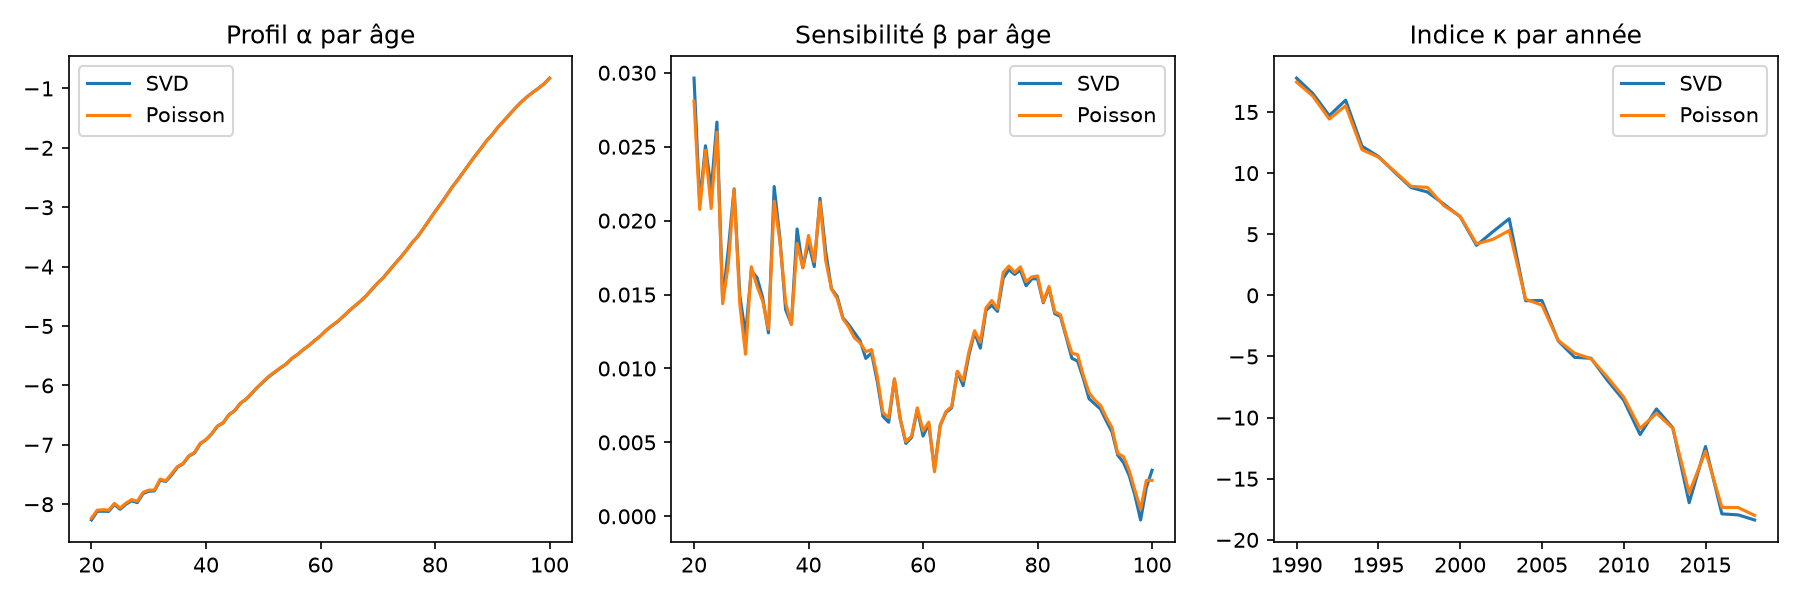
\includegraphics[width=\textwidth]{q1_parametres.png}
\caption{Paramètres de Lee--Carter obtenus par SVD réajustée et Poisson.}
\label{fig:param}
\end{figure}

Les profils $\alpha_x$ sont presque confondus et augmentent avec l'âge. Les indices $\kappa_t$ diminuent nettement, d'environ 17,5 en 1990 à $-18,0$ en 2018 pour Poisson. Comme les $\beta_x$ de cette estimation sont positifs, cette baisse traduit une amélioration de la mortalité. Les sensibilités varient selon l'âge, avec des valeurs plus fortes chez les jeunes adultes et autour de 80 ans.

Les résidus conservent cependant une structure visible, notamment une bande diagonale aux grands âges (annexe~B). Une telle diagonale suit approximativement une génération. Elle suggère une composante de cohorte que le modèle âge--période ne décrit pas explicitement. Le rapport de Pearson reste supérieur à un pour les deux méthodes. Le modèle ne résume donc pas toute la variabilité des décès, même après l'ajustement de Poisson.

Nous retenons Poisson comme méthode principale pour la suite, car elle modélise directement les décès avec leurs expositions et améliore les trois indicateurs retenus. Nous conservons les résultats SVD pour évaluer la sensibilité des prévisions et des prix au choix de la méthode d'estimation.

\newpage
\subsection{Évolution de l'indice temporel}
\subsubsection{Modèles envisagés}

Pour chacune des deux séries, nous étudions les variations $\Delta\kappa_t=\kappa_t-\kappa_{t-1}$. La première possibilité est une marche aléatoire avec dérive, $\Delta\kappa_t=d+\varepsilon_t$. La seconde autorise une dépendance entre deux variations successives,
\[
\Delta\kappa_t=c+\phi\Delta\kappa_{t-1}+\varepsilon_t,
\qquad \varepsilon_t\overset{\mathrm{iid}}\sim\mathcal N(0,\sigma^2).
\]
Il s'agit d'un AR(1) sur les variations, donc d'un modèle ARIMA(1,1,0) pour $\kappa_t$ avec dérive. Les coefficients sont estimés par régression linéaire.

\subsubsection{Diagnostics et choix du modèle temporel}

\begin{figure}[H]\centering
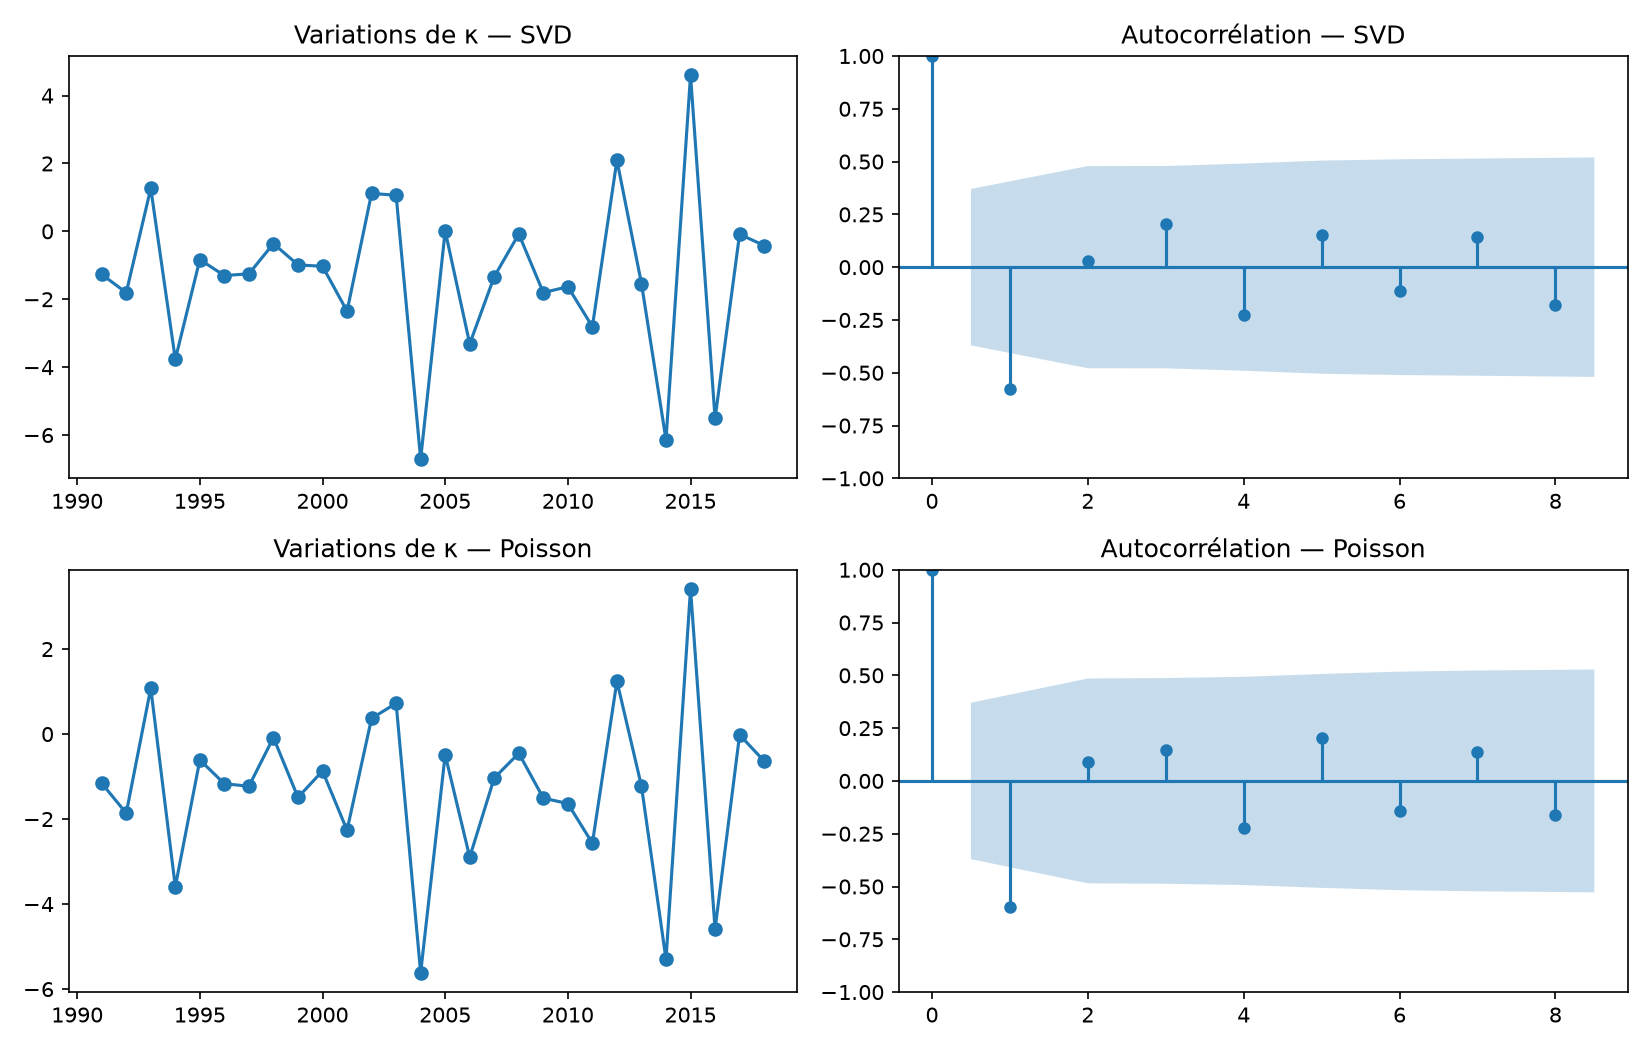
\includegraphics[width=0.56\textwidth]{q2_diagnostics.png}
\caption{Variations annuelles de $\kappa_t$ et autocorrélations empiriques.}
\label{fig:temps}
\end{figure}

Les variations présentent une alternance que la marche aléatoire ne prend pas en compte. Nous testons l'autocorrélation des résidus par Ljung--Box jusqu'au retard 5, avec la correction d'un paramètre pour l'AR(1).
\begin{table}[H]\centering\small
\caption{Estimation temporelle et diagnostics des résidus.}
\begin{tabular}{llrrrrr}\toprule
Méthode & Dynamique & $c$ ou $d$ & $\phi$ & $\sigma$ & $p_{\rm LB}$ & $p_{\rm Shapiro}$\\\midrule
SVD & Marche & $-1,291$ & 0 & 2,402 & 0,013 & 0,231\\
SVD & AR(1) & $-2,062$ & $-0,582$ & 2,032 & 0,123 & 0,552\\
Poisson & Marche & $-1,266$ & 0 & 1,956 & 0,009 & 0,310\\
Poisson & AR(1) & $-2,044$ & $-0,600$ & 1,627 & 0,185 & 0,654\\\bottomrule
\end{tabular}\label{tab:temps}
\end{table}

Au seuil de 5\,\%, Ljung--Box rejette l'absence d'autocorrélation pour les marches, mais plus pour les AR(1). Les $\phi$ négatifs, de module inférieur à un, traduisent une alternance autour de la variation moyenne $c/(1-\phi)$, soit $-1,30$ pour SVD et $-1,28$ pour Poisson. La mortalité diminue donc en moyenne. Shapiro--Wilk ne rejette pas la normalité des résidus, sous réserve du petit échantillon.

Le test ADF avec constante et tendance rejette une racine unitaire en niveau ($p=4,3\times10^{-5}$ pour SVD et $9,2\times10^{-5}$ pour Poisson), comme dans les différences. Il n'impose donc pas de différencier : une tendance déterministe serait une autre piste. Nous retenons l'AR(1) des variations parmi les deux modèles comparés pour ses résidus et sa simplicité. Avec 29 années, les prévisions restent conditionnelles à ce choix.

\newpage
\subsection{Prévision de la mortalité en 2023}
\subsubsection{Simulation et distribution par âge}

Nous simulons 10\,000 trajectoires en partant du $\kappa_{2018}$ ajusté et de la dernière variation observée. Pour chaque scénario $s$, nous tirons des innovations normales indépendantes et calculons successivement
\[
\Delta\kappa_{2018+h}^{(s)}=\widehat c+\widehat\phi\Delta\kappa_{2017+h}^{(s)}
+\varepsilon_{2018+h}^{(s)},\qquad
\kappa_{2018+h}^{(s)}=\kappa_{2017+h}^{(s)}+\Delta\kappa_{2018+h}^{(s)}.
\]
Cinq transitions conduisent de 2018 à 2023. Nous obtenons alors
\[
\mu_{x,2023}^{(s)}=\exp(\widehat\alpha_x+\widehat\beta_x\kappa_{2023}^{(s)}),
\qquad q_{x,2023}^{(s)}=1-\exp(-\mu_{x,2023}^{(s)}).
\]
Les paramètres ajustés restent fixes. La graine aléatoire 2030 permet de reproduire les résultats. Pour chaque âge, nous calculons la moyenne, l'écart-type empirique et les quantiles à 2,5\,\% et 97,5\,\%. Ces quantiles décrivent un intervalle de prévision ponctuel conditionnel au modèle, et non l'incertitude sur la seule moyenne simulée.

\begin{table}[H]\centering\small
\caption{Probabilités de décès en 2023 selon Poisson, en pourcentage.}
\begin{tabular}{rrrrr}\toprule
Âge & Moyenne & Écart-type & Quantile 2,5\,\% & Quantile 97,5\,\%\\\midrule
20 & 0,0133 & 0,0010 & 0,0115 & 0,0153\\
40 & 0,0625 & 0,0031 & 0,0566 & 0,0685\\
60 & 0,4948 & 0,0073 & 0,4804 & 0,5090\\
80 & 3,0534 & 0,1258 & 2,8111 & 3,3021\\
100 & 33,6263 & 0,1704 & 33,2888 & 33,9548\\\bottomrule
\end{tabular}
\end{table}

\begin{figure}[H]\centering
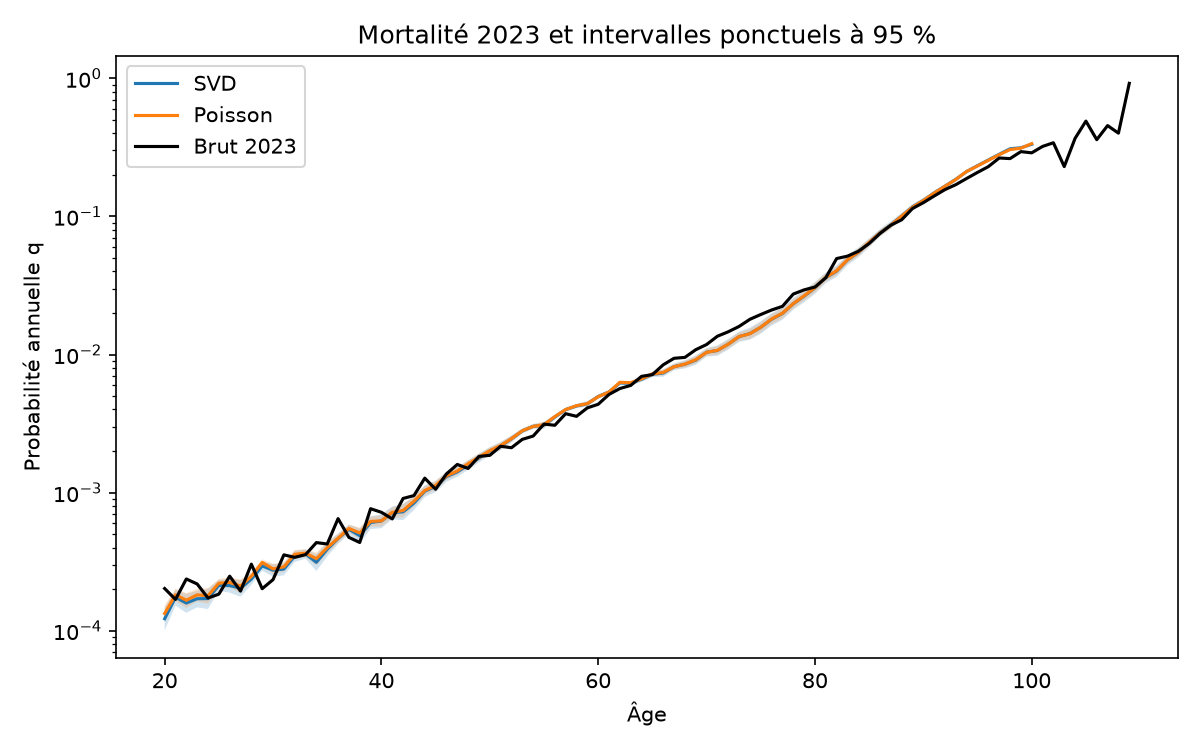
\includegraphics[width=0.75\textwidth]{q3_mortalite.png}
\caption{Probabilités prévues en 2023, intervalles ponctuels à 95\,\% et mortalité brute observée.}
\label{fig:prevision}
\end{figure}

\newpage
\subsubsection{Espérances de vie et comparaison aux observations}

Les deux méthodes donnent des courbes de mortalité proches. Les observations de 2023 restent plus irrégulières, surtout aux âges où les décès ou les expositions sont faibles. Les bandes simulées ne couvrent pas toutes ces fluctuations, puisqu'elles représentent uniquement les innovations futures de $\kappa_t$. L'incertitude d'estimation, le risque de modèle et le bruit d'observation des taux bruts ne sont pas inclus.

Comme demandé, nous construisons une table de période à partir des probabilités moyennes $\bar q_x=\frac1N\sum_s q_{x,2023}^{(s)}$. Nous utilisons la force équivalente $\bar\mu_x=-\log(1-\bar q_x)$ et calculons
\[
\mathring e_x=\sum_{j\geq0}{}_jp_x\frac{1-e^{-\bar\mu_{x+j}}}{\bar\mu_{x+j}},
\qquad {}_jp_x=\exp\left(-\sum_{r=0}^{j-1}\bar\mu_{x+r}\right).
\]
Le facteur annuel est le même que dans la partie statique et tient compte de la fraction d'année vécue l'année du décès. Cette espérance correspond à la table moyenne de 2023. Elle ne suit pas l'évolution future d'une cohorte et n'est pas la moyenne des espérances calculées scénario par scénario.

Le modèle s'arrête à 100 ans et les taux bruts annuels exploitables à 109 ans. Pour fermer chaque table, nous prolongeons la force après son dernier âge disponible selon une loi de Gompertz, $\mu_{L+h}=\mu_L e^{gh}$. La pente $g$ est estimée par régression de $\log\mu_x$ sur l'âge entre 90 et 100 ans. Nous intégrons jusqu'à 141 ans et vérifions que la survie résiduelle est inférieure à $10^{-10}$. Cette fermeture constitue une hypothèse supplémentaire. La partie statique a retenu une troncature à 105 ans, d'où de petits écarts possibles entre ses valeurs brutes et celles présentées ici.

Pour XR, nous utilisons les rapports $\ell_{x+1}/\ell_x$ et la même hypothèse de force constante à l'intérieur de chaque année. Entre 113 et 114 ans, où les derniers survivants disparaissent, nous supposons les décès uniformément répartis dans l'année.

\begin{table}[H]\centering\small
\caption{Espérances de vie de période en 2023, en années.}
\begin{tabular}{rrrrr}\toprule
Âge & Brut 2023 & SVD & Poisson & XR\\\midrule
20 & 64,463 & 64,767 & 64,737 & 61,297\\
30 & 54,590 & 54,883 & 54,859 & 51,655\\
40 & 44,808 & 45,084 & 45,064 & 42,103\\
50 & 35,273 & 35,522 & 35,509 & 32,787\\
60 & 26,137 & 26,484 & 26,474 & 23,977\\
70 & 17,699 & 18,005 & 18,003 & 16,093\\\bottomrule
\end{tabular}\label{tab:vie}
\end{table}

Poisson dépasse les valeurs brutes de 0,24 à 0,34 an selon l'âge. La prévision est donc légèrement optimiste en matière de longévité, tout en restant proche des observations. Les écarts SVD--Poisson ne dépassent pas 0,031 an. XR donne des espérances plus faibles, par exemple 23,977 ans à 60 ans contre 26,474 pour Poisson. La comparaison des rentes ci-dessous complète celle des espérances de vie.

\newpage
\subsection{Tarification d'une rente viagère temporaire}
\subsubsection{Méthode de simulation}

Nous considérons une femme âgée de 60 ans en 2018, une rente annuelle de 1\,000 euros pendant 20 ans, payable à terme échu, et un taux d'intérêt de 1,25\,\%. Nous prolongeons les trajectoires de $\kappa_t$ avec le même modèle temporel. À l'année $2018+j$, la bénéficiaire a $60+j$ ans. La force à utiliser suit donc simultanément son âge et l'année calendaire,
\[
\mu_{60+j,2018+j}^{(s)}=
\exp\left(\widehat\alpha_{60+j}+\widehat\beta_{60+j}\kappa_{2018+j}^{(s)}\right).
\]
Pour chaque trajectoire, nous calculons la probabilité de survie jusqu'au paiement $k$,
\[
{}_kp_{60,2018}^{(s)}=
\exp\left(-\sum_{j=0}^{k-1}\mu_{60+j,2018+j}^{(s)}\right),
\]
puis le prix conditionnel de la rente,
\[
P^{(s)}=1\,000\sum_{k=1}^{20}(1,0125)^{-k}\,{}_kp_{60,2018}^{(s)}.
\]
Dans le programme, la survie est initialisée à un et le prix à zéro. À chaque année, nous multiplions la survie par $e^{-\mu}$, puis ajoutons un seul paiement de 1\,000 euros pondéré par cette survie et actualisé. La boucle effectue exactement 20 ajouts. Le premier paiement survient après un an, à 61 ans. Le dernier survient après 20 ans, à 80 ans, en utilisant pour la dernière année la mortalité à 79 ans en 2037.

La moyenne des 10\,000 prix estime la valeur actuarielle sous le modèle. Leur écart-type et leurs percentiles mesurent la variation de cette valeur lorsque la trajectoire de mortalité change. Les décès individuels de la bénéficiaire ne sont pas simulés, car leur effet est déjà intégré dans les probabilités de survie.

\subsubsection{Résultats et référence XR}
\begin{table}[H]\centering\small
\caption{Distribution des valeurs actuarielles simulées, en euros.}
\begin{tabular}{lrr}\toprule
Indicateur & SVD & Poisson\\\midrule
Moyenne & 16\,266,69 & 16\,262,30\\
Écart-type & 42,98 & 34,67\\
Percentile 1\,\% & 16\,163,72 & 16\,179,89\\
Percentile 5\,\% & 16\,193,38 & 16\,203,45\\
Percentile 95\,\% & 16\,335,75 & 16\,318,28\\
Percentile 99\,\% & 16\,362,89 & 16\,340,49\\\bottomrule
\end{tabular}\label{tab:rentes}
\end{table}

Comme dans la partie statique, le prix de référence XR est obtenu directement à partir des survivants,
\[
P^{\mathrm{XR}}=1\,000\sum_{k=1}^{20}(1,0125)^{-k}\frac{\ell_{60+k}}{\ell_{60}}
=15\,384,74\ \text{euros}.
\]
Ce montant retrouve celui de la partie statique à 60 ans. La table XR étant fixe, son prix ne dépend pas de l'année de souscription dans ces calculs.

\newpage
\subsubsection{Interprétation des prix et limites}

\begin{figure}[H]\centering
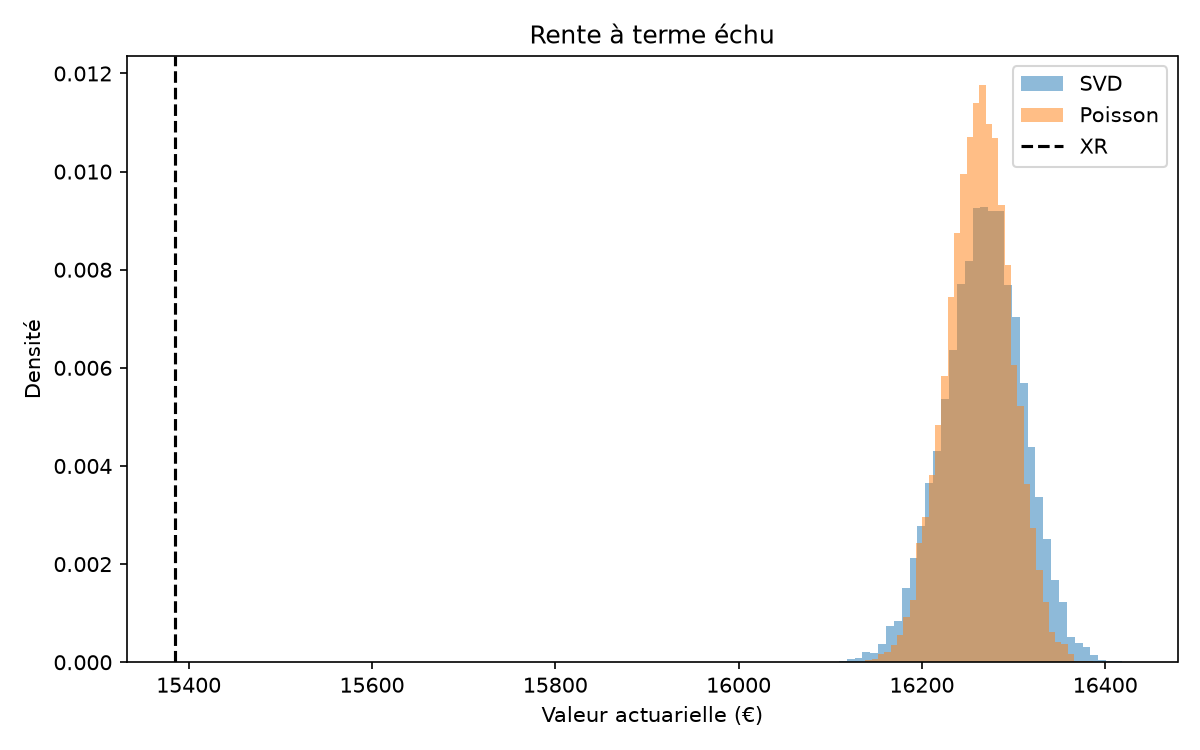
\includegraphics[width=0.75\textwidth]{q4_rentes.png}
\caption{Distribution des prix conditionnels de rente et prix de référence XR.}
\label{fig:rentes}
\end{figure}

Le prix moyen selon Poisson dépasse XR de 877,56 euros, soit environ 5,70\,\%. Pour SVD, l'écart est de 881,96 euros, soit 5,73\,\%. Les deux estimations de Lee--Carter conduisent donc pratiquement au même tarif moyen, avec seulement 4,39 euros de différence. Poisson donne toutefois une dispersion plus faible, cohérente avec un écart-type des innovations temporelles inférieur à celui de SVD.

Sous Poisson, 90\,\% des prix simulés sont compris entre 16\,203,45 et 16\,318,28 euros. La référence XR se situe bien en dessous de cette plage. Dans notre modèle, les probabilités de survie pondérées par l'actualisation conduisent donc à davantage de paiements attendus qu'avec XR. Pour une rente, une longévité plus élevée augmente le coût de la prestation.

Il faut distinguer cette dispersion d'environ 35 euros du risque total porté par un assureur. Elle concerne la valeur actuarielle conditionnelle à une trajectoire de mortalité. Elle ne comprend ni l'incertitude sur les paramètres estimés, ni les erreurs de spécification, ni l'aléa des décès individuels, ni un risque de taux. L'écart avec XR est une comparaison de tarifs et ne suffit pas, à lui seul, à vérifier une contrainte portant sur chaque probabilité de survie.

Les tarifs statiques et dynamiques n'ont pas non plus exactement le même sens. Dans la partie statique, une table de 2020 ou de 2023 est maintenue fixe pendant la rente. Ici, une souscription en 2018 est suivie avec une mortalité qui évolue pendant le contrat. Le supplément de prix ne peut donc pas être attribué uniquement à la méthode d'estimation, puisque la date de référence et les hypothèses temporelles diffèrent aussi.

\subsubsection*{Conclusion de la partie dynamique}

Poisson améliore légèrement l'ajustement de Lee--Carter et tient compte des expositions. L'AR(1) sur les variations de $\kappa_t$ corrige l'autocorrélation laissée par la marche aléatoire. Les espérances de vie prévues en 2023 restent proches des observations, avec une légère surestimation. Pour la rente, nous retenons 16\,262,30 euros selon Poisson, contre 15\,384,74 euros avec XR. Les résultats SVD sont proches, mais cette stabilité ne supprime ni l'incertitude du choix temporel ni les structures restantes des résidus.

\newpage
\appendix
\setcounter{section}{1}
\renewcommand{\thefigure}{B\arabic{figure}}
\setcounter{figure}{0}
\section{Diagnostic complémentaire du modèle dynamique}
\begin{figure}[H]\centering
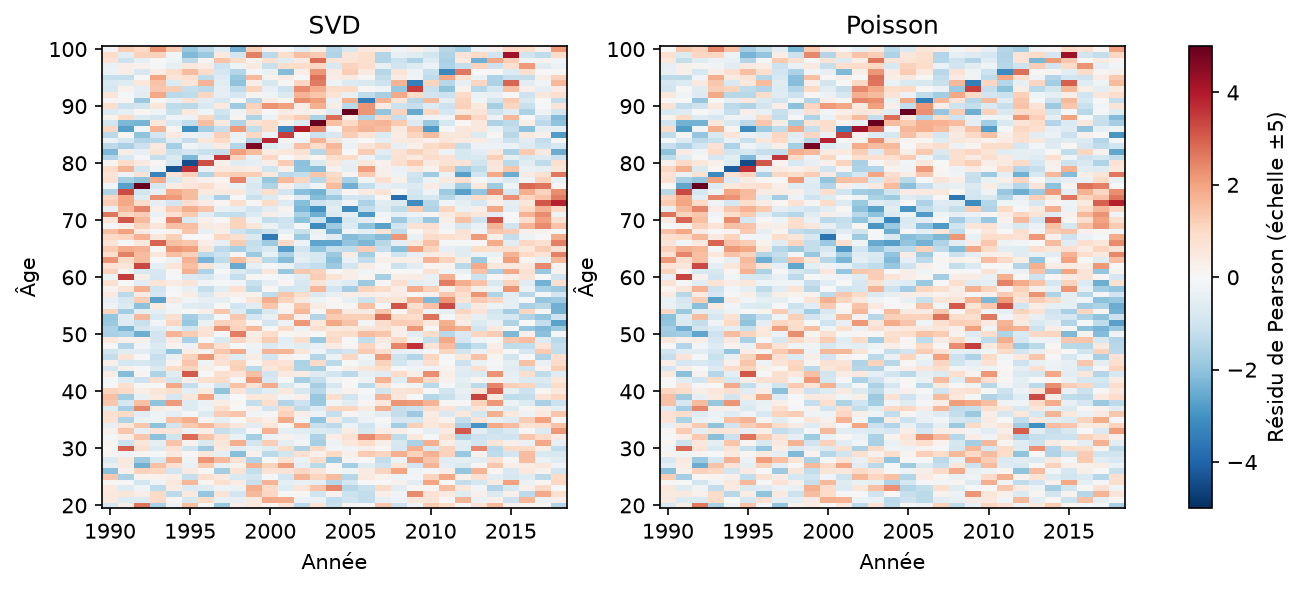
\includegraphics[width=\textwidth]{q1_residus.png}
\caption{Résidus de Pearson des décès, de 1990 à 2018 et de 20 à 100 ans. L'échelle de couleurs est limitée à $[-5,5]$.}
\label{fig:residus}
\end{figure}

Un résidu positif indique davantage de décès observés que prévu par le modèle. Un résidu négatif indique l'inverse. Les deux cartes se ressemblent fortement. La bande diagonale qui part d'environ 75 ans au début de la période et se décale vers les grands âges illustre une structure que l'indice temporel unique n'absorbe pas complètement. Une extension avec effet de cohorte pourrait être étudiée, mais elle dépasse le modèle demandé ici.

\subsection*{Sources et correspondance avec le code}

Les données de décès et d'expositions proviennent des fichiers HMD belges fournis sur Moodle. Le fichier \texttt{table\_XR.csv} reprend les valeurs de survivants de la feuille XR du classeur \texttt{TablesXRXKbrut.xlsm}. La fermeture finale à 114 ans utilise le dernier effectif nul de cette table.

Les méthodes SVD, de réajustement des décès annuels et de maximum de vraisemblance de Poisson suivent le cours LACTU2030, notamment les diapositives 177 et 181--183. Les consignes utilisées sont celles de \emph{Travail2026.pdf}, partie « Dynamic mortality modeling ».

Le fichier \texttt{partie\_dynamique.py} produit les graphiques et les tableaux employés dans ce rapport. Les fichiers \texttt{q3\_mortalite\_SVD.csv} et \texttt{q3\_mortalite\_Poisson.csv} contiennent les moyennes, écarts-types et quantiles pour tous les âges de 20 à 100 ans, pour $\mu$ et pour $q$. Le tableau de la section 2.3 en présente une sélection afin de garder le rapport lisible.
\end{document}
